%%%% SIGNAL SECTION %%%%
\section{MCS Performance on Automatically Selected Muons from numuCC Events With Cosmics in Simulation}\label{MC_performance_section}

\subsection{Input Sample}\label{MC_BNB_input_sample_section}
The input sample to this portion of the analysis is roughly 190,000 MCC7 simulated BNB neutrino interactions with CORSIKA cosmics as used by the CCInclusive group and descibed in their interal note\cite{CCIncInternalNote}. These simulated events are run through a fully automated reconstruction chain and then a fully automated event selection routine described in Section \ref{MC_BNB_eventselection_section}. The SAM definition used for this sample is ``prodgenie\_bnb\_nu\_cosmic\_uboone\_mcc7\_reco2''.

\subsection{Event Selection}\label{MC_BNB_eventselection_section}
The event selection algorithms used are designed to locate $\nu_\mu$ charged-current interactions, where at least one muon track exits the interaction vertex. The event selection is described in detail in Section 6.2.1 of the {\ub} CCInclusive internal note (``Selection IIA: track multiplicity 2 (or larger) and no containment requirement'')\cite{CCIncInternalNote}  but the main points will be recapped here. The selection takes as input reconstructed vertices created by the ``pmtrack'' producer module, reconstructed tracks created by the ``pandoraNuPMA'' track producer module, and optical hits produced by the ``opFlashSat'' producer module. The fiducial volume used in this subanalysis is the same as is used throughout the note, defined in Section \ref{fidvol_section}. The following selection cuts are placed to isolate $\nu_\mu$ charged-current interactions, and their efficiencies are documented in the aforementioned CCInclusive internal note:
\begin{enumerate}
\item The event must have at least one flash inside of the BNB beam-spill window brighter than 50 PE.
\item Two or more reconstructed tracks must originate from the same reconstructed vertex within the fiducial volume (defined in Section \ref{fidvol_section}).
\item The tracks must overlap within a 70 cm buffer in the drift (z) direction of the center of the reconstructed optical flash.
\item For events with exactly two tracks originating from the vertex, additional calorimetric-based cuts are applied to mitigate backgrounds from in-time cosmics which produce Michel electrons that get reconstructed as a track.
\end{enumerate}
%starting with 15286 events here
After these event selection cuts are placed, the sample size is 15286 events. Further cuts are placed to isolate single tracks that are eligible for this MCS analysis. 
\begin{enumerate}
\item The longest track is assumed to be the muon, and it is the only track studied in this analysis. 
\item This track must be fully contained within the fiducial volume (6384 events remain).
\item This track must be at least one meter in length (2406 events remain).
\item This track must match with an {\sc MCTrack} (Section \ref{MCTrack_section}) originating from the true neutrino interaction in the event. Here, ``match'' means that the start of the reconstructed track is within 3 cm of the start of the {\sc MCTrack}, and the end of the reconstructed track is within 3 cm of the end of the {\sc MCTrack} (or vice-versa). Note this removes any cosmic-induced mis-identifications. (1613 events remain).

\end{enumerate}

After these additional cuts are placed, 1613 events (tracks) remain for MCS analysis. It should be known that there are some inherent pion and proton mis-identification (MID) backgrounds in this sample after these cuts are placed. 88\% of the time the identified track is truly a muon. Protons and pions make up the remaining MIDs with 8.6\% and 3.4\% respectively.


% Let's be honest with ourselves this pie chart is unnecessary and should just be described in one sentence.
% \begin{figure}[ht!]
% \begin{center}
% 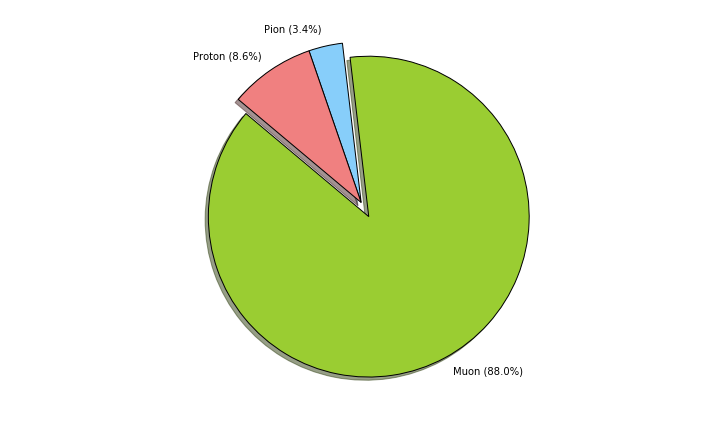
\includegraphics[width=100mm]{Figures/MCBNBSelectedRecoTrack_MID_piechart.png}
% \end{center}
% \caption{\textit{A pie chart summarizing the types and rates of different MIDs inherent in this sample. 88\% of the time the identified track is truly a muon. Protons and pions make up the remaining MID rates with 8.6\% and 3.4\% respectively.}}
% \label{MCBNBSelectedRecoTrack_MID_piechart_fig}
% \end{figure}


\subsection{MCS Momentum Validation}\label{MCS_Momentum_Validation_MCBNBSelectedRecoTrack_section}
The MCS momentum versus range-based momentum without any cuts other than those described in Section \ref{MC_BNB_eventselection_section} can be seen in Figure \ref{MCS_range_momentum_MCBNBSelectedRecoTrack_noPDGcut_fig}. The off-diagonal component visible in this figure (where MCS momentum overestimates range momentum) is caused primarily by MIDs, most commonly where the longest track is a proton. Note that there are no ``broken tracks'' (which is another not-yet-discussed possible explanation for the off-diagonal component) because of the track-{\sc MCTrack} matching requirement described in Section \ref{MC_BNB_eventselection_section}. Figure \ref{MCS_range_momentum_MCBNBSelectedRecoTrack_withPDGcuts_fig} divides Figure \ref{MCS_range_momentum_MCBNBSelectedRecoTrack_noPDGcut_fig} into those events in which the MCTrack matched to the reconstructed track is a proton, a pion, or a muon. From this figure it is clear comparing MCS momentum to range momentum for contained tracks will provide a handle on separating muon tracks from proton tracks in data (though it is hard to make similar conclusions about pions due to limited statistics in this study).\\

The bias and resolution for the MCS momentum estimation method on this sample is computed in the same way as described in previous sections (for example in Section \ref{MCS_Momentum_Validation_MCBNBRecoTrack_section}). Note that only those events in which the reconstructed track corresponds to a muon in truth (Figure \ref{MCS_range_momentum_MCBNBSelectedRecoTrack_muononly_fig}) are used to compute bias and resolutions. The bias and resolution for this momentum reconstruction method is shown in Figure \ref{MCS_range_bias_resolution_MCBNBSelectedRecoTrack_fig}. This figure indicates a bias in the MCS momentum resolution on the order of a few percent, with a resolution that decreases from about 10\% for contained tracks with true total momentum around 0.5 GeV (which corresponds to a length of about 1.7 meters) to below 7\% for contained tracks with true total momentum greater than 0.8 GeV (which corresponds to a length of about 3.1 meters). This agrees well with the analogous plots created from simulated single muons with reconstructed tracks (Figure \ref{MCS_range_bias_resolution_MCBNBRecoTrack_fig}).


\begin{figure}[ht!]
\begin{center}
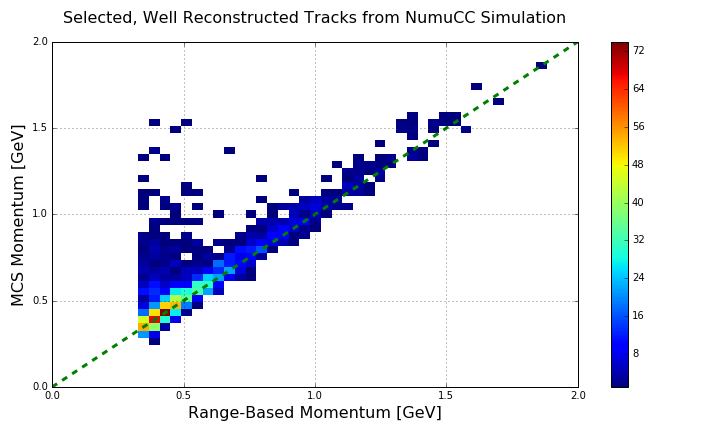
\includegraphics[width=100mm]{Figures/MCS_range_comparison_MCBNBSelectedRecoTrack.png}
\end{center}
\caption{\textit{MCS computed momentum versus range momentum for the automatically selected simulated neutrino-induced fully contained, well reconstructed muon sample without any additional cuts to mitigate MIDs.}}
\label{MCS_range_momentum_MCBNBSelectedRecoTrack_noPDGcut_fig}
\end{figure}

\begin{figure}
\centering
\mbox{
	\subfigure[\textit{The subset of events in Figure \ref{MCS_range_momentum_MCBNBSelectedRecoTrack_noPDGcut_fig} in which the true identity of the track is a proton.}]
	{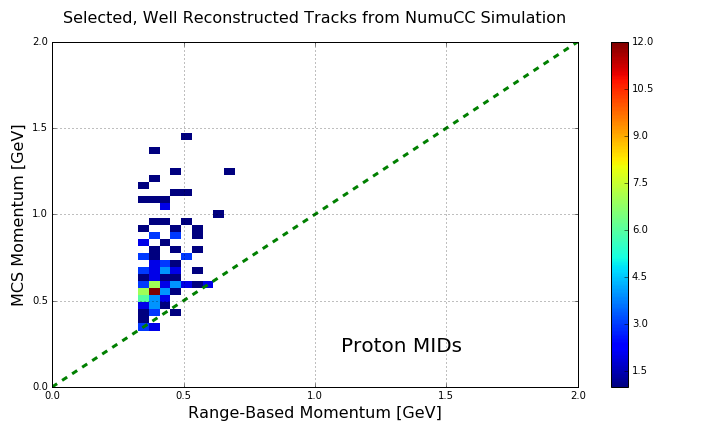
\includegraphics[width=50mm]{Figures/MCS_range_momentum_MCBNBSelectedRecoTrack_2212.png}}
	\quad
	\subfigure[\textit{The subset of events in Figure \ref{MCS_range_momentum_MCBNBSelectedRecoTrack_noPDGcut_fig} in which the true identity of the track is a pion.}]
	{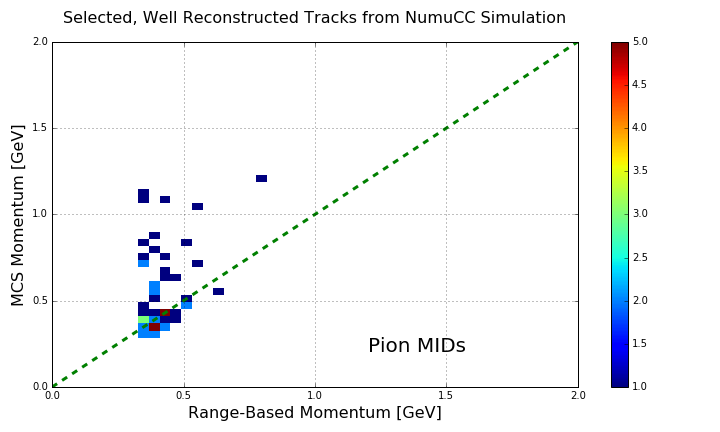
\includegraphics[width=50mm]{Figures/MCS_range_momentum_MCBNBSelectedRecoTrack_211.png}}
	\quad
	\subfigure[\textit{The subset of events in Figure \ref{MCS_range_momentum_MCBNBSelectedRecoTrack_noPDGcut_fig} in which the true identity of the track is a muon.}\label{MCS_range_momentum_MCBNBSelectedRecoTrack_muononly_fig}]
	{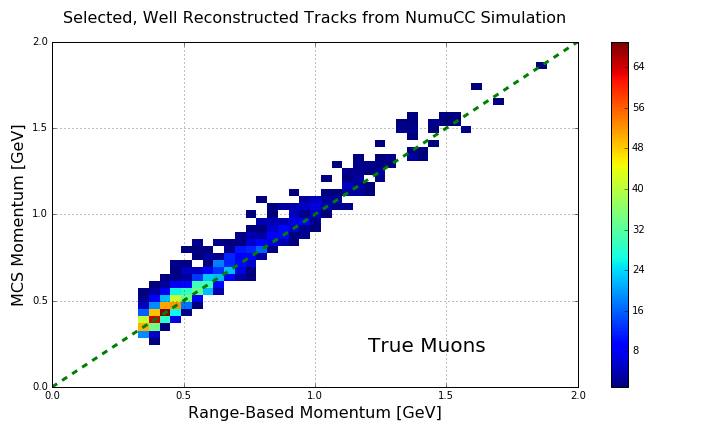
\includegraphics[width=50mm]{Figures/MCS_range_momentum_MCBNBSelectedRecoTrack_13.png}}
	}
\caption{\textit{MCS computed momentum versus range momentum for the selected neutrino-induced, well reconstructed fully contained muon sample in simulation broken up by true particle identity of the track.}}
\label{MCS_range_momentum_MCBNBSelectedRecoTrack_withPDGcuts_fig}
\end{figure}


\begin{figure}
\centering
\mbox{
	\subfigure[\textit{Fractional momentum difference between 0.35 and 0.53 GeV range momentum.}]
	{\includegraphics[width=50mm]{Figures/{MCS_range_resolution_MCBNBSelectedRecoTrack_slice_0.35_0.53}.png}}
	\quad
	\subfigure[\textit{Fractional momentum difference between 0.90 and 1.08 GeV range momentum.}]
	{\includegraphics[width=50mm]{Figures/{MCS_range_resolution_MCBNBSelectedRecoTrack_slice_0.90_1.08}.png}}
	\quad
	\subfigure[\textit{Fractional momentum difference between 1.45 and 1.63 GeV range momentum.}]
	{\includegraphics[width=50mm]{Figures/{MCS_range_resolution_MCBNBSelectedRecoTrack_slice_1.45_1.63}.png}}
	}

\caption{\textit{Fractional momentum difference for a few representative bins of range momentum derived from Figure \ref{MCS_range_momentum_MCBNBSelectedRecoTrack_muononly_fig} (which is produced using only those tracks which truly match to a muon).}}
\label{MCS_range_bias_resolution_MCBNBSelectedRecoTrack_slices_fig}
\end{figure}


\begin{figure}
\centering
\mbox{
	\subfigure[\textit{MCS momentum bias as a function of range momentum. The vertical error bars are computed as $\frac{\sigma_{fit}}{\sqrt{N}}$, and the horizontal error bars indicate bin width.}]
	{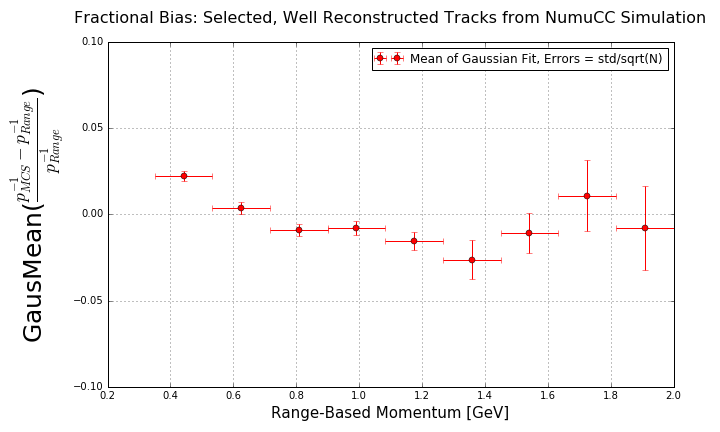
\includegraphics[width=75mm]{Figures/MCS_range_bias_MCBNBSelectedRecoTrack.png}}
	\quad
	\subfigure[\textit{MCS momentum resolution as a function of range momentum. The vertical error bars are computed as $\frac{\sigma_{fit}}{\sqrt{2N}}$, and the horizontal error bars indicate bin width.}]
	{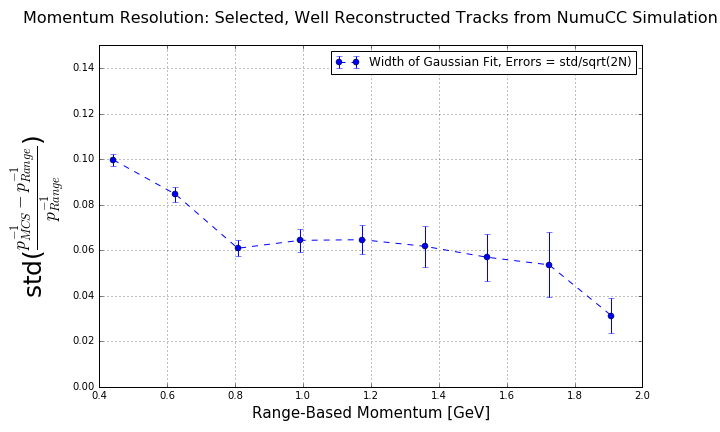
\includegraphics[width=75mm]{Figures/MCS_range_resolution_MCBNBSelectedRecoTrack.png}}
	}
\caption{\textit{MCS momentum bias and resolution as a function of range momentum for the selected, well reconstructed neutrino-induced muons in {\ub} simulation.}}
\label{MCS_range_bias_resolution_MCBNBSelectedRecoTrack_fig}
\end{figure}



\subsection{Highland Validation}\label{Highland_Validation_MCBNBSelectedRecoTrack_section}
For this sample of contained, automatically selected, well-reconstructed neutrino-induced tracks, the same Highland validation plot is created in exactly the same way as described in Section \ref{Highland_Validation_MCTrack_section}. For each consecutive pair of segments, the angular scatter in milliradians divided by the Highland expected RMS in millradians is an entry in the histogram shown in Figure \ref{Highland_validation_MCBNBSelectedRecoTracks_fig}. From this figure we can see that the Highland formula is valid for automatically selected, well reconstructed neutrino-induced muon tracks in simulation.

\begin{figure}[ht!]
\begin{center}
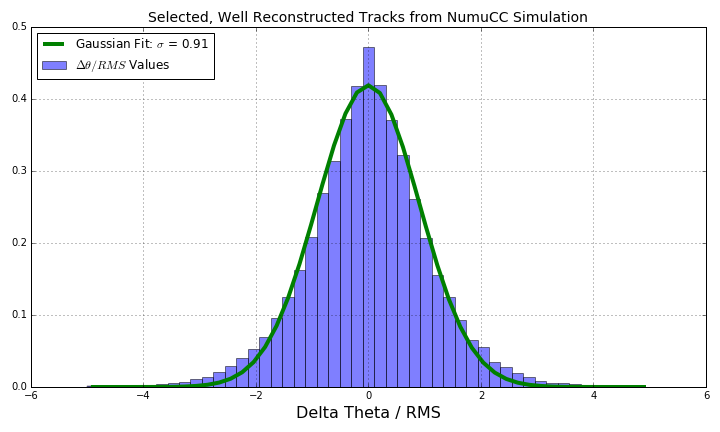
\includegraphics[width=100mm]{Figures/Highland_validation_MCBNBSelectedRecoTrack.png}
\end{center}
\caption{\textit{10 cm segment angular deviations divided by expected Highland RMS for the sample of well reconstructed, neutrino induced muons in simulation.}}
\label{Highland_validation_MCBNBSelectedRecoTracks_fig}
\end{figure}